\documentclass{standalone}
\usepackage{tikz}
\usetikzlibrary{patterns, positioning}


\begin{document}
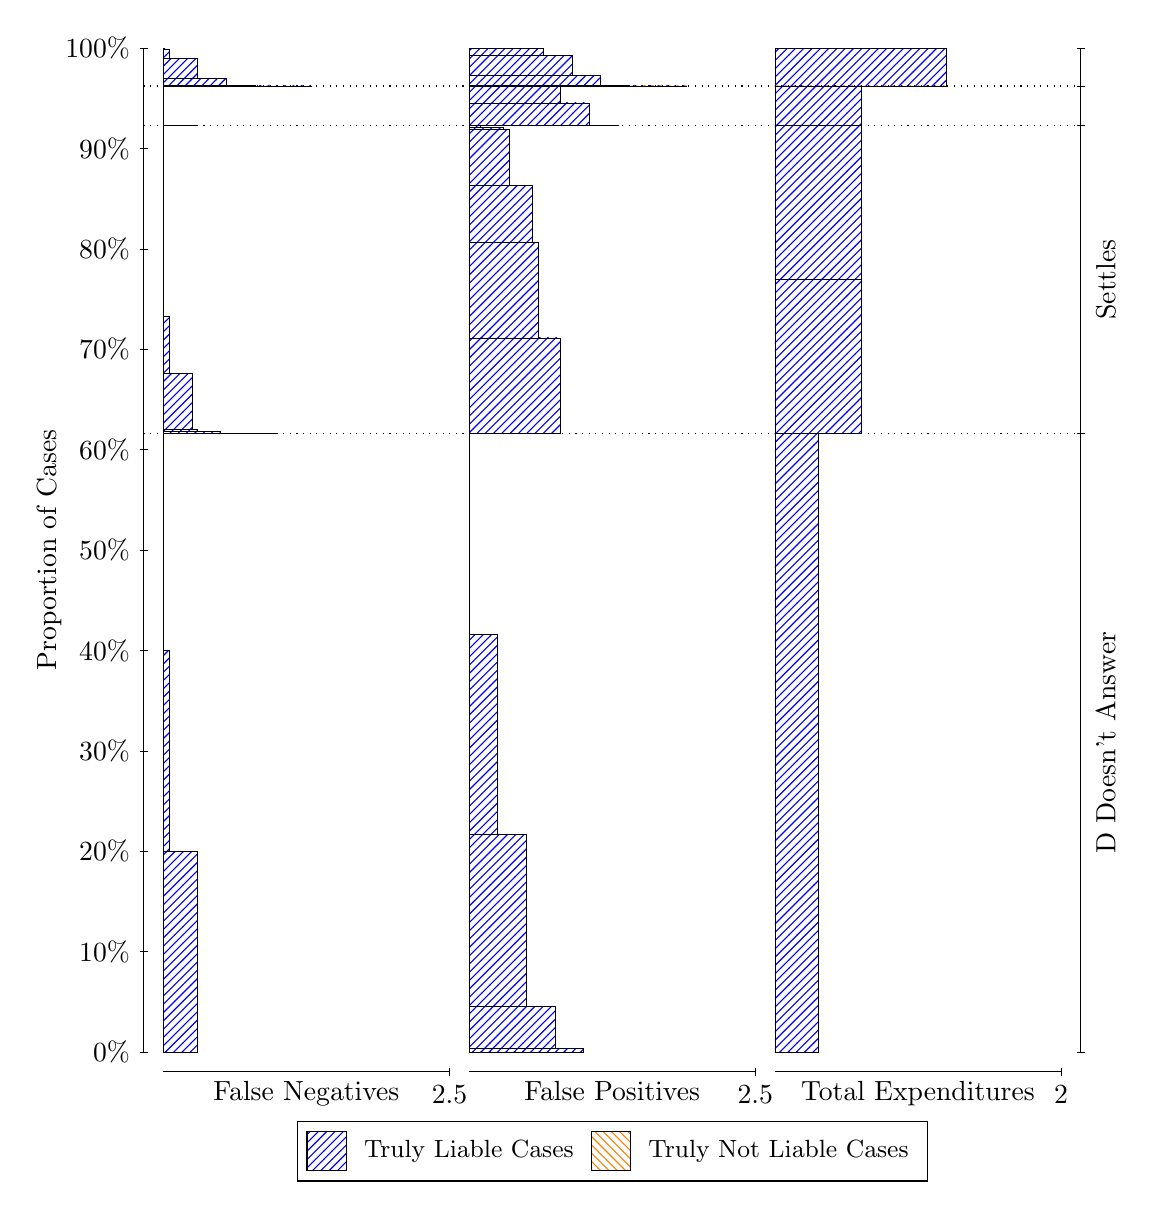
\begin{tikzpicture}
\draw[black, very thin] (1.5,1.75) -- (1.5,14.5);
\node[rotate=90, text=black, anchor=center] at (0.3, 8.125) {Proportion of Cases};
\draw[black, very thin] (1.45,1.75) -- (1.55,1.75);
\node[text=black, anchor=east] at (1.45, 1.75) {0\%};
\draw[black, very thin] (1.45,3.025) -- (1.55,3.025);
\node[text=black, anchor=east] at (1.45, 3.025) {10\%};
\draw[black, very thin] (1.45,4.3) -- (1.55,4.3);
\node[text=black, anchor=east] at (1.45, 4.3) {20\%};
\draw[black, very thin] (1.45,5.575) -- (1.55,5.575);
\node[text=black, anchor=east] at (1.45, 5.575) {30\%};
\draw[black, very thin] (1.45,6.85) -- (1.55,6.85);
\node[text=black, anchor=east] at (1.45, 6.85) {40\%};
\draw[black, very thin] (1.45,8.125) -- (1.55,8.125);
\node[text=black, anchor=east] at (1.45, 8.125) {50\%};
\draw[black, very thin] (1.45,9.4) -- (1.55,9.4);
\node[text=black, anchor=east] at (1.45, 9.4) {60\%};
\draw[black, very thin] (1.45,10.675) -- (1.55,10.675);
\node[text=black, anchor=east] at (1.45, 10.675) {70\%};
\draw[black, very thin] (1.45,11.95) -- (1.55,11.95);
\node[text=black, anchor=east] at (1.45, 11.95) {80\%};
\draw[black, very thin] (1.45,13.225) -- (1.55,13.225);
\node[text=black, anchor=east] at (1.45, 13.225) {90\%};
\draw[black, very thin] (1.45,14.5) -- (1.55,14.5);
\node[text=black, anchor=east] at (1.45, 14.5) {100\%};

\draw[black, very thin] (13.4,1.75) -- (13.4,14.5);
\draw[black, very thin] (13.35,1.75) -- (13.45,1.75);
\node[anchor=west] at (13.35, 1.75) {};
\draw[black, very thin] (13.35,9.6076) -- (13.45,9.6076);
\node[anchor=west] at (13.35, 9.6076) {};
\draw[black, very thin] (13.35,13.514) -- (13.45,13.514);
\node[anchor=west] at (13.35, 13.514) {};
\draw[black, very thin] (13.35,14.018) -- (13.45,14.018);
\node[anchor=west] at (13.35, 14.018) {};
\draw[black, very thin] (13.35,14.5) -- (13.45,14.5);
\node[anchor=west] at (13.35, 14.5) {};

\draw[black, very thin, pattern color=blue, pattern=north east lines] (1.75,1.75) rectangle (2.186,4.2999);
\draw[black, very thin, pattern color=blue, pattern=north east lines] (1.75,4.2999) rectangle (1.8227,6.8468);
\draw[black, very thin, pattern color=orange, pattern=north west lines] (1.75,6.8468) rectangle (1.75,6.8468);
\draw[black, very thin, pattern color=blue, pattern=north east lines] (1.75,6.8468) rectangle (1.75,9.6076);
\draw[black, very thin, pattern color=blue, pattern=north east lines] (1.75,9.6076) rectangle (3.2033,9.6076);
\draw[black, very thin, pattern color=blue, pattern=north east lines] (1.75,9.6076) rectangle (2.9127,9.6076);
\draw[black, very thin, pattern color=blue, pattern=north east lines] (1.75,9.6076) rectangle (2.84,9.6076);
\draw[black, very thin, pattern color=blue, pattern=north east lines] (1.75,9.6076) rectangle (2.5493,9.6076);
\draw[black, very thin, pattern color=blue, pattern=north east lines] (1.75,9.6076) rectangle (2.4767,9.6315);
\draw[black, very thin, pattern color=blue, pattern=north east lines] (1.75,9.6315) rectangle (2.186,9.6559);
\draw[black, very thin, pattern color=blue, pattern=north east lines] (1.75,9.6559) rectangle (2.1133,10.37);
\draw[black, very thin, pattern color=blue, pattern=north east lines] (1.75,10.37) rectangle (1.8227,11.093);
\draw[black, very thin, pattern color=orange, pattern=north west lines] (1.75,11.093) rectangle (1.75,11.093);
\draw[black, very thin, pattern color=blue, pattern=north east lines] (1.75,11.093) rectangle (1.75,13.514);
\draw[black, very thin, pattern color=blue, pattern=north east lines] (1.75,13.514) rectangle (2.186,13.514);
\draw[black, very thin, pattern color=blue, pattern=north east lines] (1.75,13.514) rectangle (1.8227,13.516);
\draw[black, very thin, pattern color=orange, pattern=north west lines] (1.75,13.516) rectangle (1.75,13.516);
\draw[black, very thin, pattern color=blue, pattern=north east lines] (1.75,13.516) rectangle (1.75,14.018);
\draw[black, very thin, pattern color=blue, pattern=north east lines] (1.75,14.018) rectangle (3.6393,14.018);
\draw[black, very thin, pattern color=blue, pattern=north east lines] (1.75,14.018) rectangle (3.276,14.018);
\draw[black, very thin, pattern color=blue, pattern=north east lines] (1.75,14.018) rectangle (2.9127,14.021);
\draw[black, very thin, pattern color=blue, pattern=north east lines] (1.75,14.021) rectangle (2.5493,14.115);
\draw[black, very thin, pattern color=blue, pattern=north east lines] (1.75,14.115) rectangle (2.186,14.115);
\draw[black, very thin, pattern color=blue, pattern=north east lines] (1.75,14.115) rectangle (2.186,14.37);
\draw[black, very thin, pattern color=blue, pattern=north east lines] (1.75,14.37) rectangle (1.8227,14.37);
\draw[black, very thin, pattern color=blue, pattern=north east lines] (1.75,14.37) rectangle (1.8227,14.488);
\draw[black, very thin, pattern color=orange, pattern=north west lines] (1.75,14.488) rectangle (1.75,14.488);
\draw[black, very thin, pattern color=blue, pattern=north east lines] (1.75,14.488) rectangle (1.75,14.5);
\draw[black, very thin, pattern color=orange, pattern=north west lines] (5.6333,1.75) rectangle (7.0867,1.75);
\draw[black, very thin, pattern color=blue, pattern=north east lines] (5.6333,1.75) rectangle (7.0867,1.7916);
\draw[black, very thin, pattern color=blue, pattern=north east lines] (5.6333,1.7916) rectangle (6.7233,2.3338);
\draw[black, very thin, pattern color=blue, pattern=north east lines] (5.6333,2.3338) rectangle (6.36,4.5108);
\draw[black, very thin, pattern color=blue, pattern=north east lines] (5.6333,4.5108) rectangle (5.9967,7.0576);
\draw[black, very thin, pattern color=blue, pattern=north east lines] (5.6333,7.0576) rectangle (5.6333,9.6076);
\draw[black, very thin, pattern color=orange, pattern=north west lines] (5.6333,9.6076) rectangle (6.796,9.6076);
\draw[black, very thin, pattern color=blue, pattern=north east lines] (5.6333,9.6076) rectangle (6.796,10.818);
\draw[black, very thin, pattern color=orange, pattern=north west lines] (5.6333,10.818) rectangle (6.5053,10.818);
\draw[black, very thin, pattern color=blue, pattern=north east lines] (5.6333,10.818) rectangle (6.5053,12.028);
\draw[black, very thin, pattern color=blue, pattern=north east lines] (5.6333,12.028) rectangle (6.4327,12.752);
\draw[black, very thin, pattern color=blue, pattern=north east lines] (5.6333,12.752) rectangle (6.142,13.465);
\draw[black, very thin, pattern color=blue, pattern=north east lines] (5.6333,13.465) rectangle (6.0693,13.49);
\draw[black, very thin, pattern color=blue, pattern=north east lines] (5.6333,13.49) rectangle (5.7787,13.514);
\draw[black, very thin, pattern color=blue, pattern=north east lines] (5.6333,13.514) rectangle (5.706,13.514);
\draw[black, very thin, pattern color=blue, pattern=north east lines] (5.6333,13.514) rectangle (5.6333,13.514);
\draw[black, very thin, pattern color=orange, pattern=north west lines] (5.6333,13.514) rectangle (7.5227,13.514);
\draw[black, very thin, pattern color=blue, pattern=north east lines] (5.6333,13.514) rectangle (7.5227,13.522);
\draw[black, very thin, pattern color=blue, pattern=north east lines] (5.6333,13.522) rectangle (7.1593,13.802);
\draw[black, very thin, pattern color=blue, pattern=north east lines] (5.6333,13.802) rectangle (6.796,14.016);
\draw[black, very thin, pattern color=blue, pattern=north east lines] (5.6333,14.016) rectangle (6.4327,14.018);
\draw[black, very thin, pattern color=blue, pattern=north east lines] (5.6333,14.018) rectangle (6.0693,14.018);
\draw[black, very thin, pattern color=orange, pattern=north west lines] (5.6333,14.018) rectangle (8.3947,14.018);
\draw[black, very thin, pattern color=blue, pattern=north east lines] (5.6333,14.018) rectangle (8.3947,14.018);
\draw[black, very thin, pattern color=orange, pattern=north west lines] (5.6333,14.018) rectangle (8.0313,14.018);
\draw[black, very thin, pattern color=blue, pattern=north east lines] (5.6333,14.018) rectangle (8.0313,14.018);
\draw[black, very thin, pattern color=orange, pattern=north west lines] (5.6333,14.018) rectangle (7.668,14.018);
\draw[black, very thin, pattern color=blue, pattern=north east lines] (5.6333,14.018) rectangle (7.668,14.03);
\draw[black, very thin, pattern color=orange, pattern=north west lines] (5.6333,14.03) rectangle (7.3047,14.03);
\draw[black, very thin, pattern color=blue, pattern=north east lines] (5.6333,14.03) rectangle (7.3047,14.148);
\draw[black, very thin, pattern color=orange, pattern=north west lines] (5.6333,14.148) rectangle (6.9413,14.148);
\draw[black, very thin, pattern color=blue, pattern=north east lines] (5.6333,14.148) rectangle (6.9413,14.403);
\draw[black, very thin, pattern color=blue, pattern=north east lines] (5.6333,14.403) rectangle (6.578,14.497);
\draw[black, very thin, pattern color=blue, pattern=north east lines] (5.6333,14.497) rectangle (6.2147,14.5);
\draw[black, very thin, pattern color=blue, pattern=north east lines] (5.6333,14.5) rectangle (5.8513,14.5);
\draw[black, very thin, pattern color=blue, pattern=north east lines] (5.6333,14.5) rectangle (5.6333,14.5);
\draw[black, very thin, pattern color=orange, pattern=north west lines] (9.5167,1.75) rectangle (10.062,1.75);
\draw[black, very thin, pattern color=blue, pattern=north east lines] (9.5167,1.75) rectangle (10.062,9.6076);
\draw[black, very thin, pattern color=orange, pattern=north west lines] (9.5167,9.6076) rectangle (10.607,9.6076);
\draw[black, very thin, pattern color=blue, pattern=north east lines] (9.5167,9.6076) rectangle (10.607,11.566);
\draw[black, very thin, pattern color=orange, pattern=north west lines] (9.5167,11.566) rectangle (10.607,11.566);
\draw[black, very thin, pattern color=blue, pattern=north east lines] (9.5167,11.566) rectangle (10.607,13.514);
\draw[black, very thin, pattern color=orange, pattern=north west lines] (9.5167,13.514) rectangle (10.607,13.514);
\draw[black, very thin, pattern color=blue, pattern=north east lines] (9.5167,13.514) rectangle (10.607,14.018);
\draw[black, very thin, pattern color=orange, pattern=north west lines] (9.5167,14.018) rectangle (11.697,14.018);
\draw[black, very thin, pattern color=blue, pattern=north east lines] (9.5167,14.018) rectangle (11.697,14.5);
\draw[black, dotted] (1.5,9.6076) -- (13.4,9.6076);
\draw[black, dotted] (1.5,13.514) -- (13.4,13.514);
\draw[black, dotted] (1.5,14.018) -- (13.4,14.018);
\draw[black, very thin] (1.75,1.5) -- (5.3833,1.5);
\node[text=black, anchor=north] at (3.5667, 1.5) {False Negatives};
\draw[black, very thin] (5.3833,1.45) -- (5.3833,1.55);
\node[text=black, anchor=north] at (5.3833, 1.45) {2.5};

\draw[black, very thin] (5.6333,1.5) -- (9.2667,1.5);
\node[text=black, anchor=north] at (7.45, 1.5) {False Positives};
\draw[black, very thin] (9.2667,1.45) -- (9.2667,1.55);
\node[text=black, anchor=north] at (9.2667, 1.45) {2.5};

\draw[black, very thin] (9.5167,1.5) -- (13.15,1.5);
\node[text=black, anchor=north] at (11.333, 1.5) {Total Expenditures};
\draw[black, very thin] (13.15,1.45) -- (13.15,1.55);
\node[text=black, anchor=north] at (13.15, 1.45) {2};

\node[text=black, centered, rotate=90] at (13.72, 5.6788) {D Doesn't Answer};
\node[text=black, centered, rotate=90] at (13.72, 11.561) {Settles};



\draw (7.449999999999999,1.5) node[draw=none] (baseCoordinate) {};
\begin{scope}[align=center]
        \matrix[scale=0.5, draw=black, below=0.5cm of baseCoordinate, nodes={draw}, column sep=0.1cm]{
            \node[rectangle, draw, minimum width=0.5cm, minimum height=0.5cm, pattern color=blue, pattern=north east lines] {}; &
            \node[draw=none, font=\small, text=black] (B) {Truly Liable Cases}; &
            \node[rectangle, draw, minimum width=0.5cm, minimum height=0.5cm, pattern color=orange, pattern=north west lines] {}; &
            \node[draw=none, font=\small, text=black] (B) {Truly Not Liable Cases}; \\
            };
\end{scope}

\end{tikzpicture}
\end{document}